\begin{frame}{Le geste de lecture}
    \begin{itemize}
        \item Le texte importe parfois moins que le livre qui le contient
        \item Le livre, en tant que média, s'est fait transparent (sécularisation)
        \item Le livre engage une sensorialité forte (matérialité)
        \item L'acte de lecture est indissociable de ses gestes (aspect kinésique)
    \end{itemize}
\end{frame}

\begin{frame}{Livre et tablette tactile : vers l'ux design}
    Comment les éditeurs, écrivains, designers, exploitent-ils le potentiel de la tablette tactile, en réinvestissant la dimension kinésique du livre - dimension à la fois pratique et imaginaire ?\\
    \vspace{2em}
        \textbf{Cas de l'UX Design}\\
        = la conception orientée vers l'expérience de l'utilisateur\\
        \textrightarrow{} Tenir compte de ses attentes, voire anticiper la manière dont il va naviguer sur le site, intéragir ou réagir aux fonctionnalités et apparences.\\
\end{frame}

\begin{frame}{Le design skeuomorphique}
    \begin{columns}[T,onlytextwidth]
        \column{0.50\linewidth}
        \vspace{2em}
        \small
        \begin{itemize}
        \item Néologisme formé de \textit{skeuos} (équipement militaire, mais aussi costume, ornement, décoration) pour désigner "un élément de design ou une structure qui ne sert aucun but dans l'objet formé à partir du nouveau matériau, mais qui était essentiel dans l'objet fait à partir du matériau original" (George Basalla)
        \item Ex: les premières bibliothèques Ibook
    \end{itemize}

        \column{0.50\linewidth}
        \centering
        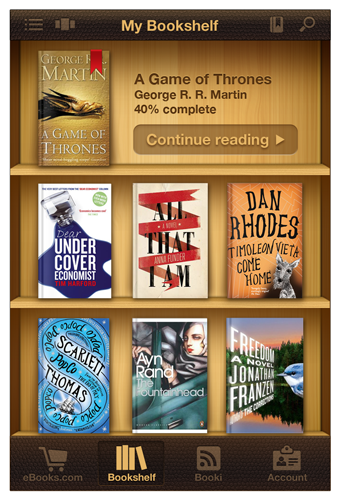
\includegraphics[width=.90\columnwidth]{Images/skeuomorphism.png}
    \end{columns}
    
\end{frame}

\begin{frame}{Le design skeuomorphique}
    \textrightarrow{} Envisageait déjà le processus de remédiation comme réitération d'un geste.\\
    \textrightarrow{} Enjeu: reproduire les gestes de lecture\\
    \textrightarrow{} Lire c'est agir, pas seulement regarder (matérialité performative)
\end{frame}

\begin{frame}{Les affordances du livre}
    \begin{block}{}
        Selon James Jerome Gibson (psychologue), l'affordance = ensemble de toutes les possibilités d'action d'un environnement.\\
     \textbf{Exemple:} face au livre imprimé traditionnel, on aura tendance à tourner les pages une par une. Mais, selon les cultures, l'ordre des pages peut changer. Ce n'est pas un "universalisme"
    \end{block}
    \begin{block}{Lire: un savoir "naturellement" produit par le médium?}
        \begin{itemize}
            \item Affordances = potentiel d'action d'un environnement tel qu'il est perçu par l'usager
            \item la notion d'affordance relie cette perfomativité à la matérialité du texte (ce que Johanna Drucker a aussi appelé la "matérialité performative")
        \end{itemize}
    \end{block}
\end{frame}
\begin{frame}{Les affordances du livre}
    \centering
    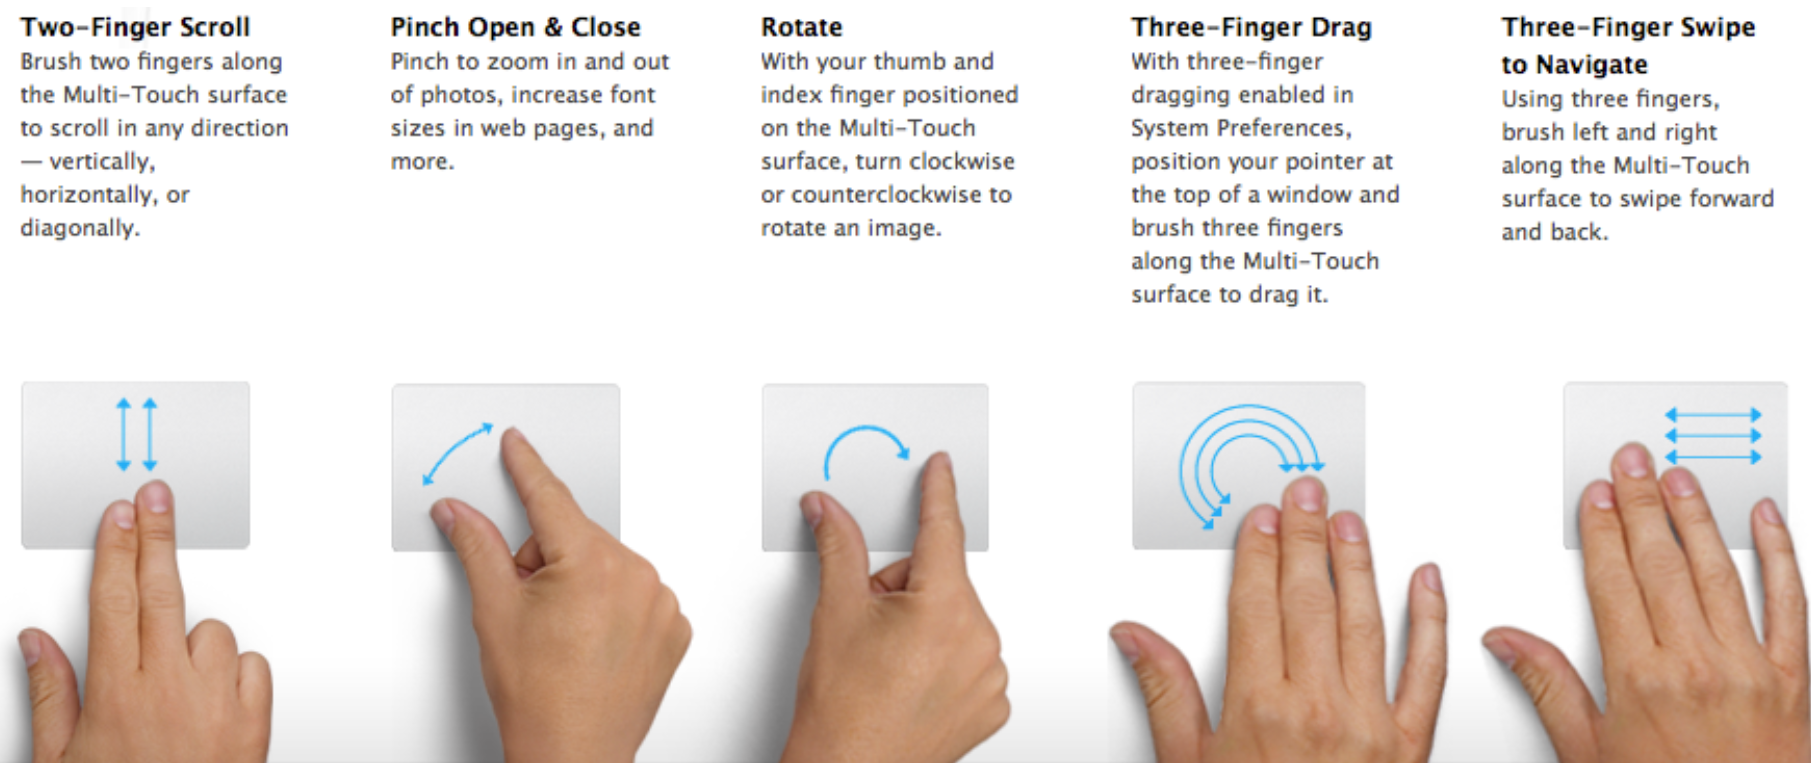
\includegraphics[width=.80\textwidth]{Images/affordances.png}
\end{frame}

\begin{frame}{La remédiation comme réitération d'un geste}
    \textrightarrow{} Réinvestir des gestes bien connus: l'expérience kinésique du livre.\\
    \begin{block}{Le champ de bataille des gestes de lecture}
        Pb : faire ces gestes suppose un travail technique que l'on néglige souvent alors qu'il est décisif.\\
        \begin{itemize}
            \item Apple vs IOS: en 2011, Apple dépose un abstract sur la technologie multitouch.
            \item Des technologies propriétaires (dans des gestes "sous embargo")
            \item Si un.e développeur.se souhaite rendre disponible une application sur Android ET ios, il devra réaliser deux version.
        \end{itemize}
    \end{block}
    \textrightarrow{} Une interface, pour qu’elle soit efficace, doit être la plus ergonomique et la plus intuitive possible pour son usager, dont les pratiques varient en fonction du contexte d’utilisation (Anaïs Guilet, 2016)
\end{frame}